% !TEX root = ../thesis.tex
\section{The Dataflow Graph Design}
\label{sec:vg:dataflow}

\vspace{-10pt}

Dataflow operators are instantiated and connected by the Reactive Vega
\emph{parser}, which traverses a declarative specification containing
definitions for input datasets, visual encoding rules, and interaction
primitives as described in~\cref{sec:vg:lang}. When data tuples are observed, or
when interaction events occur, they are propagated (or ``\emph{pulsed}'')
through the graph with each operator being evaluated in turn. Propagation ends
at the renderer.

\vspace{-10pt}

\subsection{Data, Interaction, and Scene Graph Operators}

\vspace{-7pt}

Reactive Vega's dataflow operators fall into one of three categories: input data
processing, interaction handling, or scene graph construction.

\vspace{-10pt}

\subsubsection{Processing Input Data}

\vspace{-10pt}

Reactive Vega parses each dataset definition and constructs a corresponding
branch in the dataflow graph. These branches comprise input and output nodes
connected by a pipeline of data transformation operators. Input nodes receive
raw tuples as a linear stream (tree and graph structures are supported via
parent-child or neighbor pointers, respectively). Upon data source updates,
tuples are flagged as either \emph{added}, \emph{modified}, or \emph{removed},
and each tuple is given a unique identifier. Data transformation operators use
this metadata to perform targeted computation and, in the process, may derive
new tuples from existing ones. Derived tuples retain access to their ``parent''
via prototypal inheritance\,---\,operators need not propagate unrelated upstream
changes.

Some operators require additional inspection of tuple state. Consider an
aggregate operator that calculates running statistics over a dataset (e.g.,
mean and variance). When the operator observes added or removed tuples, the
statistics can be updated based on the current tuple values. With modified
tuples, the previous value must be subtracted from the calculation and the new
value added. Correspondingly, tuples include a \texttt{previous} property.
Writes to a tuple attribute are done through a setter function that copies
current values to the \texttt{previous} object.

\subsubsection{Handling Interaction}

\vspace{-10pt}

Reactive Vega instantiates an event listener node for each low-level event type
required by the visualization (e.g., \texttt{mousedown} or \texttt{touchstart}).
These nodes are directly connected to dependent signals as specified by event
selectors~\cite{satyanarayan:declarative}. In the case of ordered selectors
(e.g., ``drag'' events specified by \texttt{[mousedown, mouseup] > mousemove}),
each constituent event is connected to an automatically created anonymous
signal; an additional anonymous signal connects them to serve as a gatekeeper,
and only propagates the final signal value when appropriate. Individual signals
can be dependent on multiple event nodes and/or other signals, and value
propagation follows E-FRP's two-phase update (\secref{sec:propagation}).

\vspace{-10pt}

\subsubsection{Constructing the Scene Graph}

\vspace{-10pt}

To construct the scene graph, Reactive Vega follows a process akin to the
Protovis bind-build-evaluate pipeline~\cite{heer:protovisjava}. When a
declarative specification is parsed, Reactive Vega traverses the mark hierarchy
to \emph{bind} property definitions: property sets are compiled into encoding
functions and stored with the specification. At run-time, \emph{build} and
\emph{evaluate} operators are created for each bound mark. The build operator
performs a data join~\cite{bostock:d3} to generate one scene graph element (or
``mark'') per tuple in the backing dataset, and the evaluate operator runs the
appropriate encoding functions. A downstream \emph{bounds} operator calculates
the bounding boxes of generated marks. For a nested scene graph to be rendered
correctly, the order of operations is critical: parent marks must be built and
encoded before their children, but the bounds of the children must be calculated
before their parents. The resultant scene graph, as seen in
\cref{fig:vg:groupedBar}, exhibits an alternating structure, with individual
mark elements grouped under a sentinel mark specification node.

\begin{figure}[t!]
  \centering
  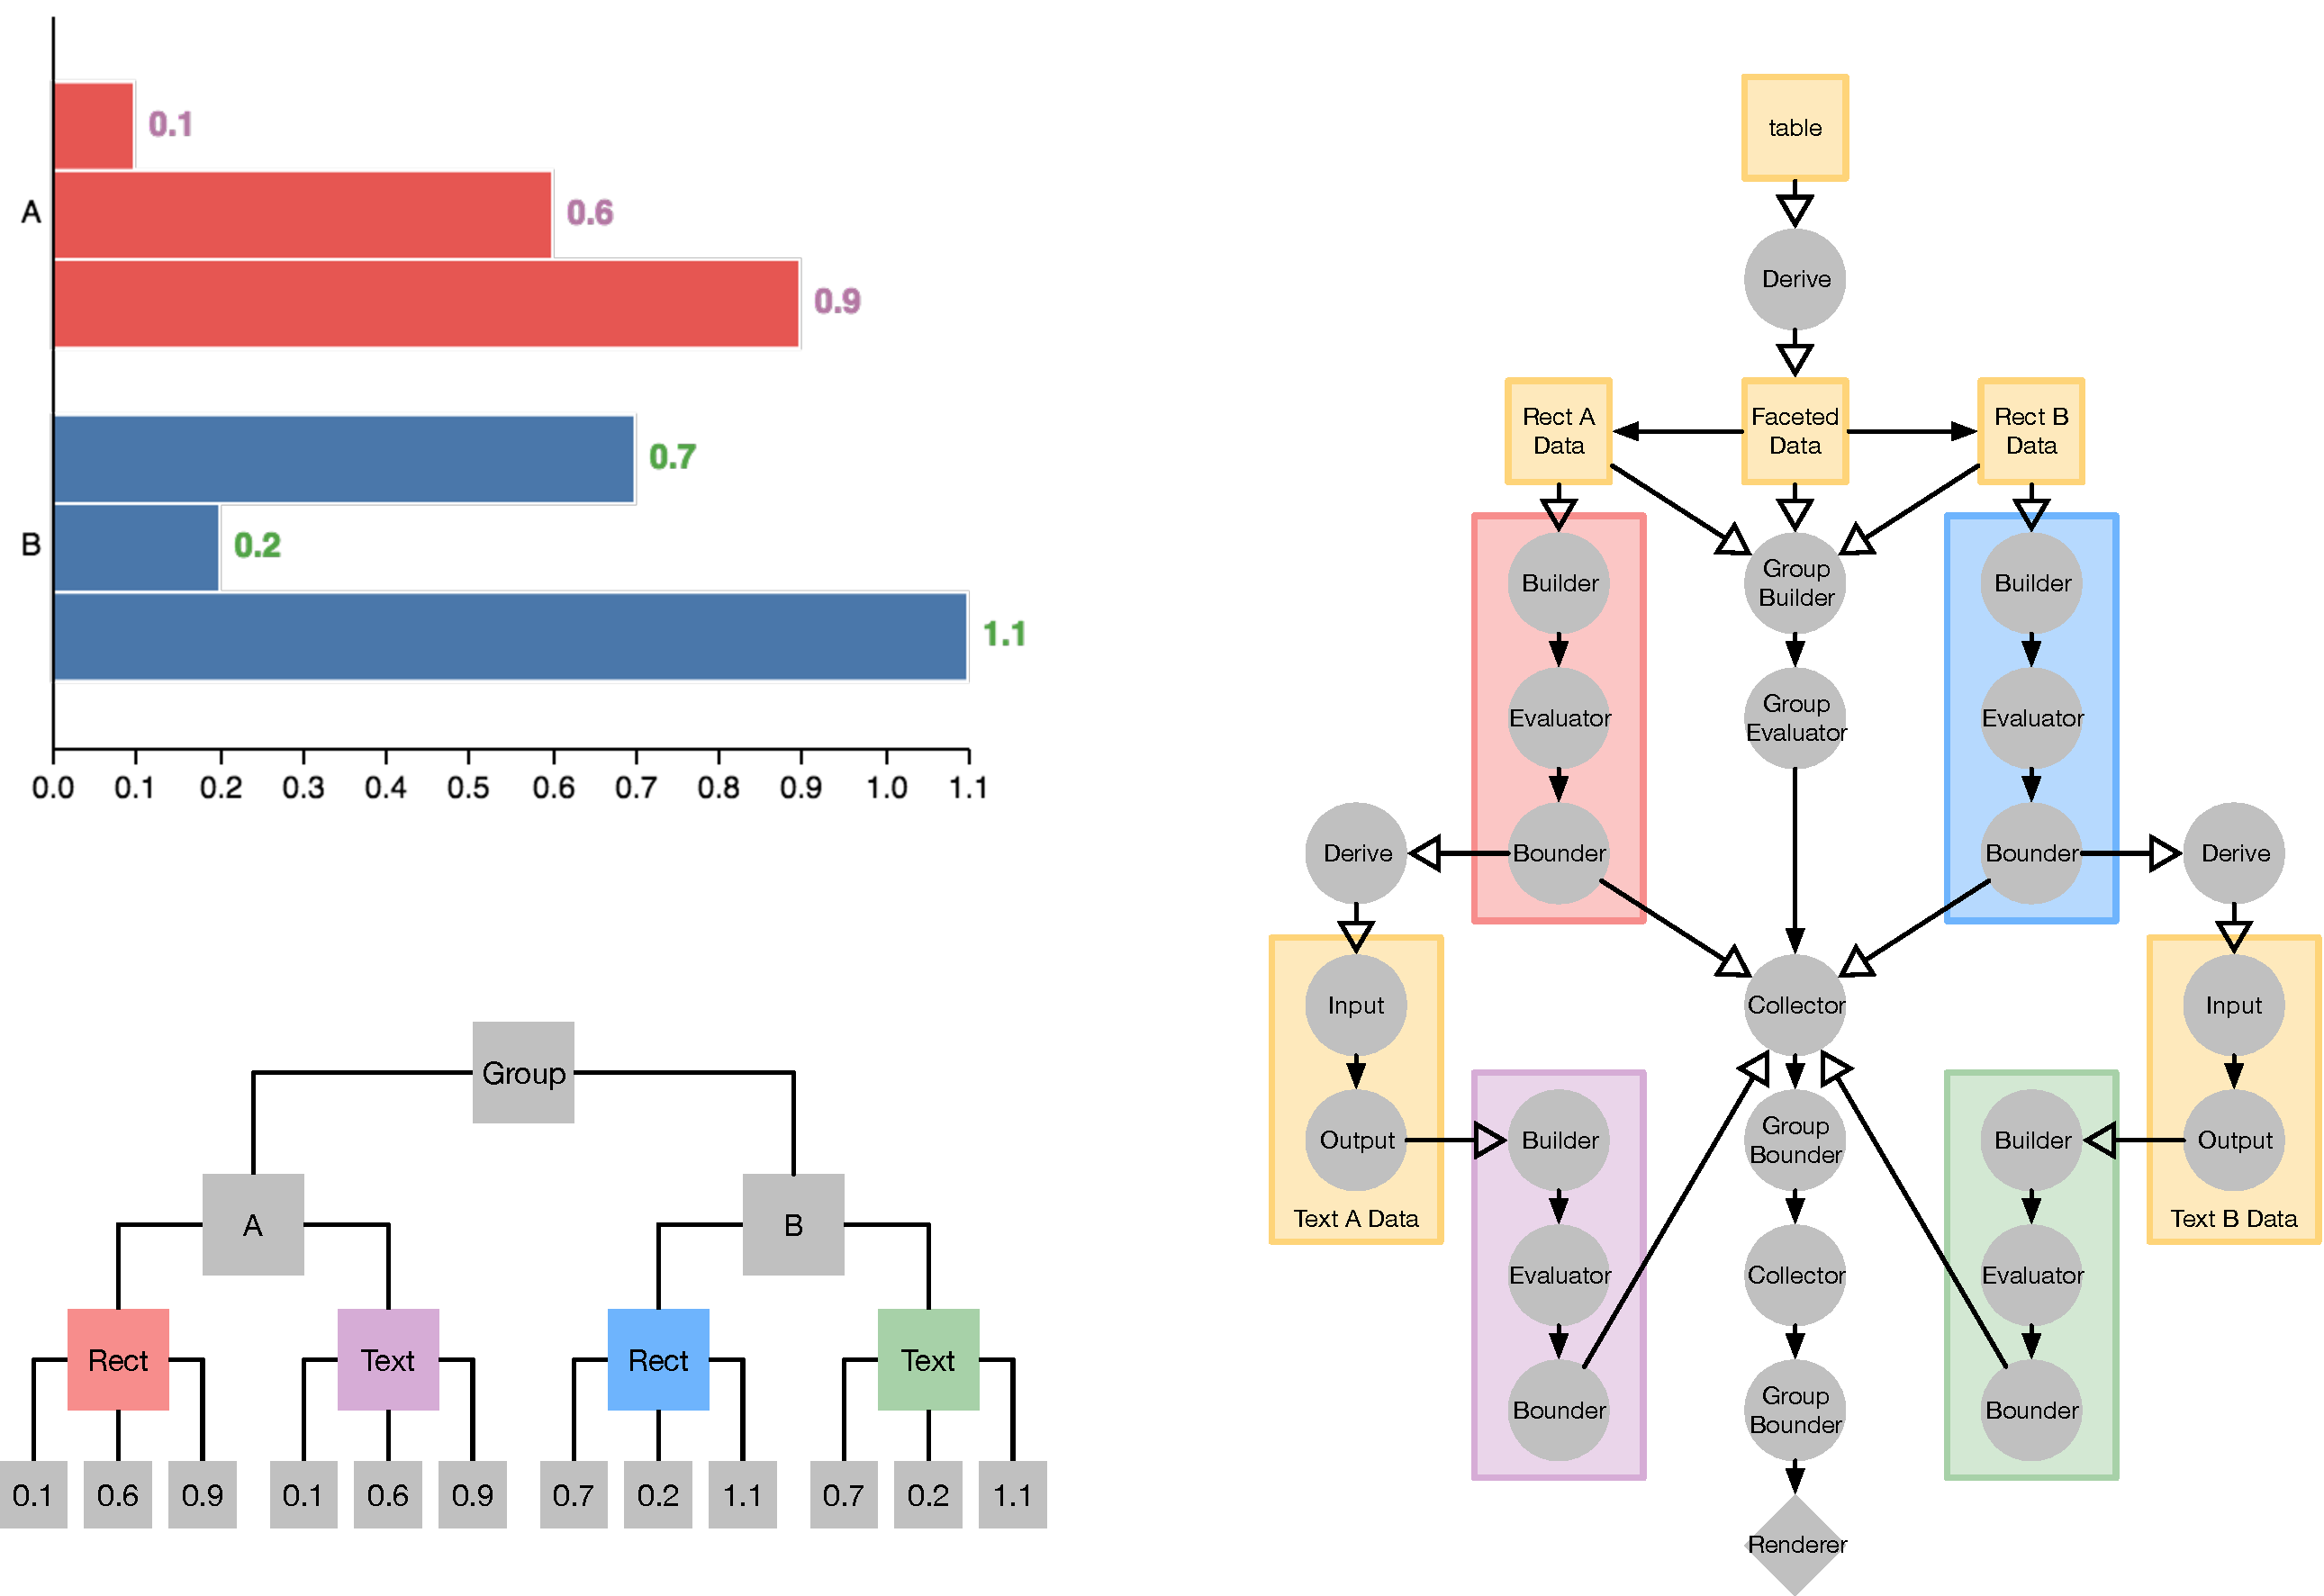
\includegraphics[width=0.9\columnwidth]{groupedBar}
  \caption{A grouped bar chart (top), with the underlying scene graph (bottom),
  and corresponding portion of the dataflow graph (right).}
  \label{fig:vg:groupedBar}
\end{figure}

Scene graph elements are also modeled as data tuples and can serve as the input
data for downstream visual encoding primitives. This establishes a
\emph{reactive geometry} that accelerates common layout tasks, such as label
positioning, and expands the expressiveness of the specification language. As
marks can be run through subsequent data transformations, higher-level layout
algorithms (e.g., those that require a pre-computed initial
layout~\cite{flexbox}) are now supported in a fully declarative fashion.

\subsection{Changesets and Materialization}

\vspace{-7pt}

All data does not flow through the system at all times. Instead, operators
receive and transmit \emph{changesets}. A changeset consists of observed tuples,
new signal values, and updates to other dependencies that have transpired since
the last render event. The propagation of a changeset begins in response to
streaming tuples or user interaction. The corresponding input node creates a
fresh changeset, and populates it with the detected update. As the changeset
flows through the graph, operators use it to perform targeted recomputation, and
may augment it in a variety of ways. For example, a \texttt{Filter} operator
might remove tuples from a changeset if they do not meet the filter predicate,
or may mark modified tuples as \texttt{added} if they previously had been
filtered. A Cartesian product operator, on the other hand, replaces incoming
tuples with the cross-product with another data stream.

Some operators, however, require a complete dataset. For example, a
windowed-join requires access to all tuples in the current windows of the joined
data sources. For such scenarios, special \emph{collector} operators (akin to
\emph{views}~\cite{abadi:aurora} or \emph{synopses}~\cite{arasu:stream} in
streaming databases) materialize the data currently in a branch. In order to
mitigate the associated time and memory expenses, Reactive Vega automatically
shares collectors between dependent operators. Upon instantiation, such
operators must be annotated as requiring a collector; at run-time they can then
request a complete dataset from the scheduler.

Finally, if animated transitions are specified, a changeset contains an
interpolation queue to which mark evaluators add generated mark instances; the
interpolators are then run when the changeset is evaluated by the renderer.

\vspace{-10pt}

\subsection{Coordinating Changeset Propagation}
\label{sec:propagation}

\vspace{-7pt}

A centralized dataflow graph scheduler is responsible for dispatching changesets
to appropriate operators. The scheduler ensures that changeset propagation
occurs in topological order so that an operator is only evaluated after all of
its dependencies are up-to-date. This schedule prevents wasteful intermediary
computation or momentary inconsistencies, known as
\emph{glitches}~\cite{cooper:embedding}. Centralizing this responsibility,
rather than delegating it to operators, enables more aggressive pruning of
unnecessary computation as described in~\secref{sec:pruning}. The scheduler has
access to the full graph structure and, thus, more insight into the state of
individual operators and propagation progress.

When an interaction event occurs, however, an initial non-topological update of
signals is performed. Dependent signals are reevaluated according to their
specification order. As a result, signals may use prior computed values of their
dependencies, which will subsequently be updated. This process mimics E-FRP's
two-phase update~\cite{wan:efrp}, and is necessary to enable expressive signal
composition. Once all necessary signals have been reevaluated, a changeset with
the new signal values is propagated to the rest of the dataflow graph.

\subsection{Pushing Internal and Pulling External Changesets}

\vspace{-7pt}

Two types of edges connect operators in the dataflow graph. The first connects
operators that work with the same data; for example a pipeline of data
transformation operators for the same data source, or a mark's build and
evaluate operators. Changesets are pushed along these edges, and operators
use and augment them directly.

The second type of edge connects operators with external dependencies (e.g.,
other data sources, signals, and scale functions). As these edges connect
disparate data spaces, they cannot directly connect operators with their
dependencies. To do so would result in operators performing computation over
mismatched data types. Instead, external dependencies are connected to their
dependents' nearest upstream \texttt{Collector} node, and changesets that flow
along these edges are flagged as \emph{reflow changesets}. When a
\texttt{Collector} receives a reflow changeset, it propagates its tuples
forward, flagging them as modified. The dependents now receive correct input
data.

Reflow changes also flow along edges that connect signals to other signals.
However, as these edges exist in scalar data space, \texttt{Collector} nodes are
not needed.

This hybrid push/pull system enables a complex web of interdependent operators
while reducing the complexity of individual elements. For example, regardless of
whether a signal parameterizes data transforms or visual encoding primitives, it
simply needs to output a reflow changeset. Without such a system in place, the
signal would instead have to construct a different changeset for each dependency
edge it was a part of, and determine the correct dataset to supply.
\Cref{fig:vg:teaser,fig:vg:groupedBar,fig:vg:scenegraph} use filled and unfilled
arrows for internal and external connections, respectively.

\vspace{-10pt}

\subsection{Dynamically Restructuring the Graph}

\vspace{-7pt}

To support streaming nested data structures, operators can dynamically
restructure the graph at runtime by extending new branches, or pruning
existing ones, based on observed data. These dataflow branches model their
corresponding hierarchies as standard relations, thereby enabling subsequent
operators to remain agnostic to higher-level structure. For example, a
\texttt{Facet} operator partitions tuples by key fields; each partition then
propagates down a unique, dynamically-constructed dataflow branch, which can
include other operators such as \texttt{Filter} or \texttt{Sort}.

In order to maintain interactive performance, new branches are queued for
evaluation as part of the same cycle they were created in. To ensure changeset
propagation continues to occur in topological order, operators are given a
\emph{rank} upon instantiation to uniquely identify their place in the ordering.
When new edges are added to the dataflow graph, the ranks are updated such that
an operator's rank is always greater than those of its dependencies. When the
scheduler queues operators for propagation, it also stores the ranks it
observes. Before propagating a changeset to an operator, the scheduler compares
the operator's current rank to the stored rank. If the ranks match, the operator
is evaluated; if the ranks do not match, the graph was restructured and the
scheduler requeues the operator.

\begin{figure}[t!]
  \centering
  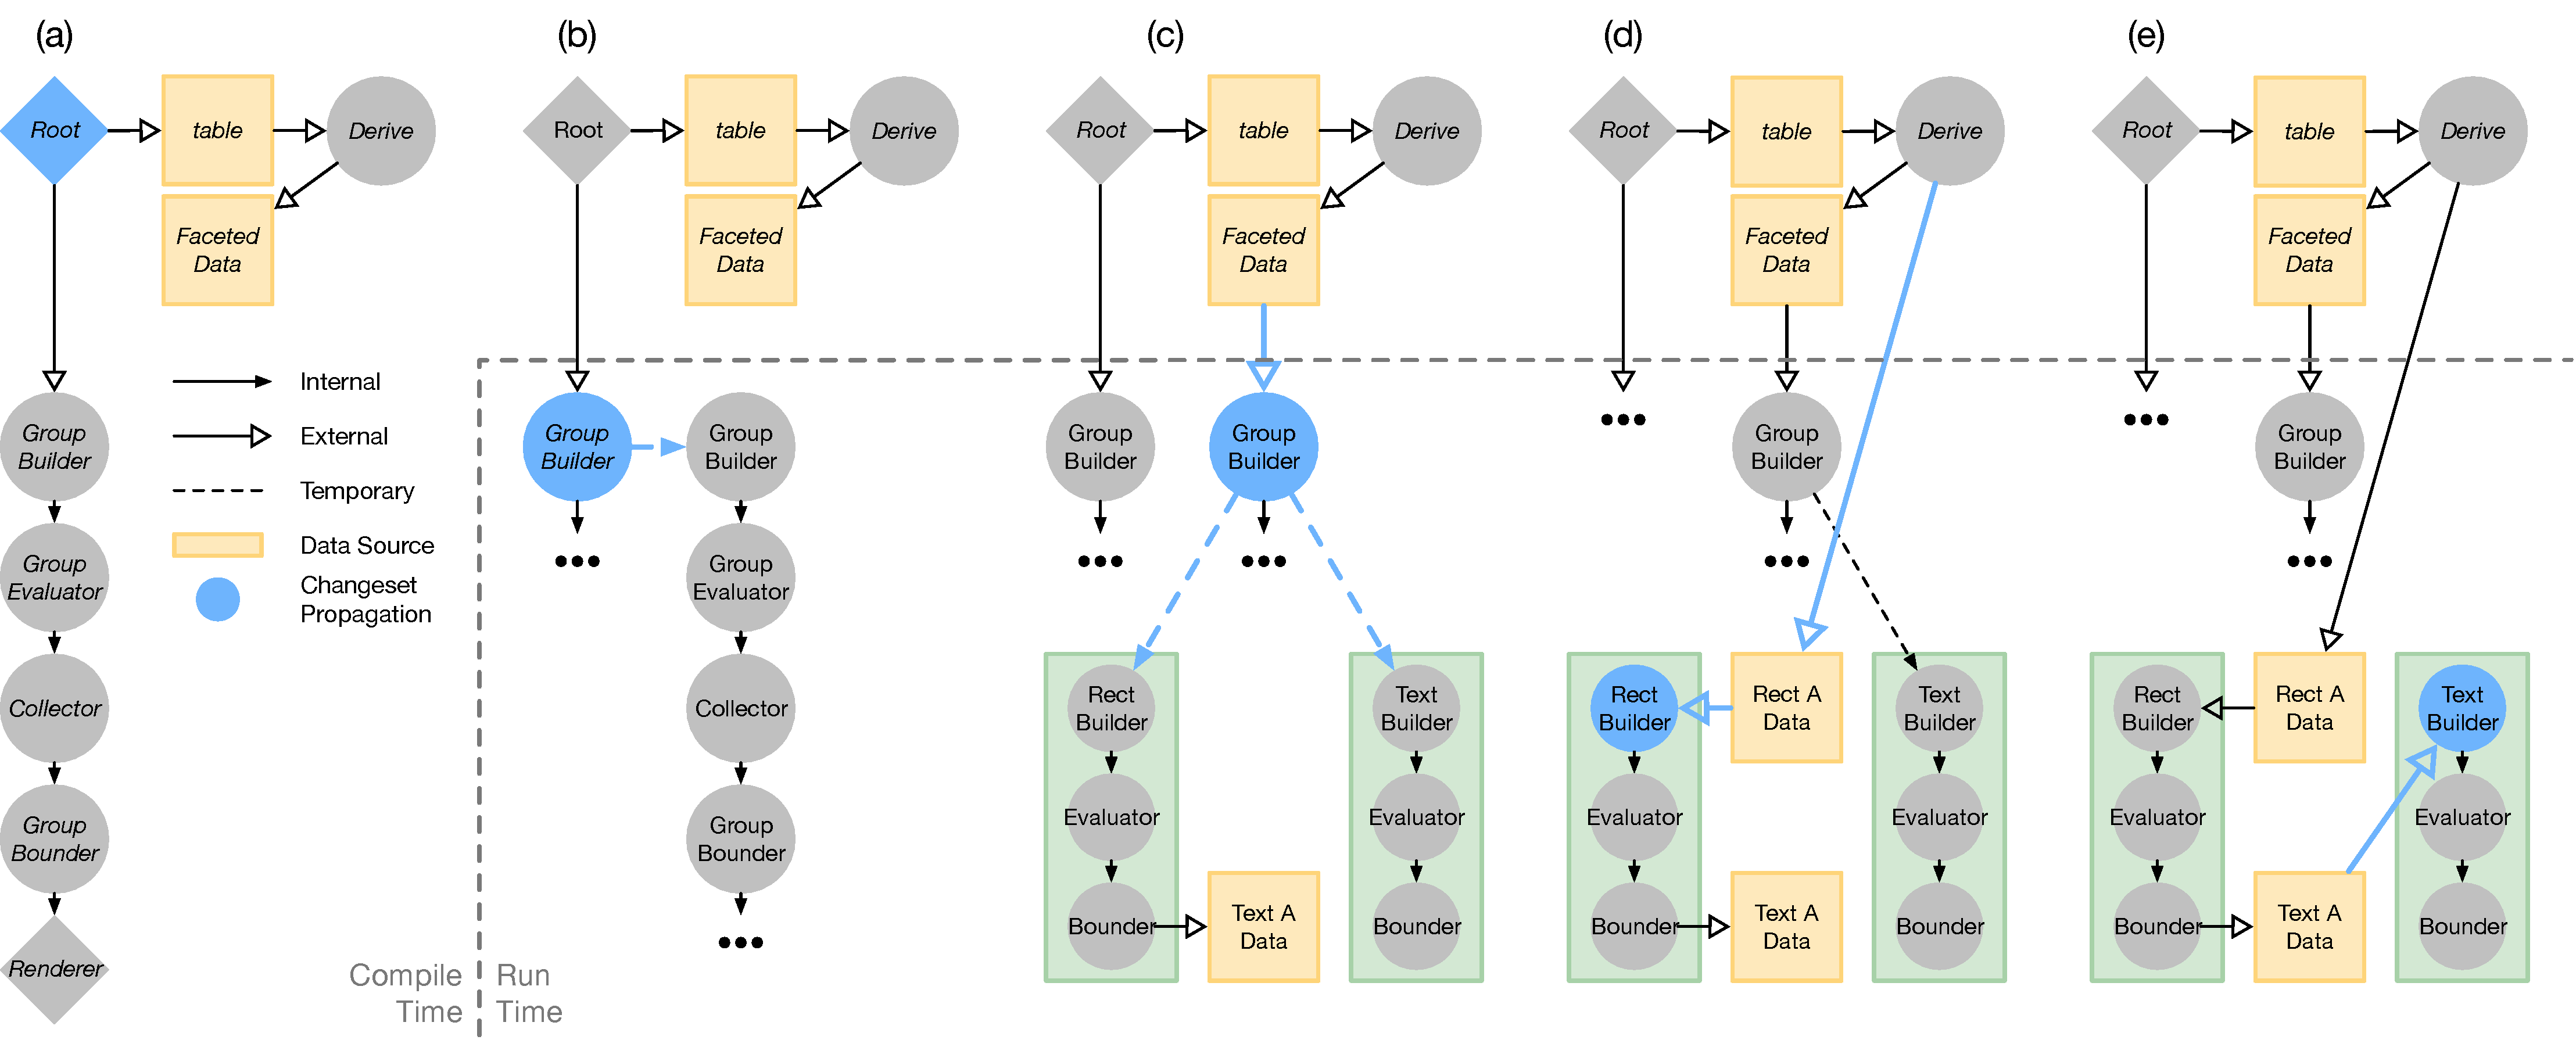
\includegraphics[width=\columnwidth]{scenegraph}
  \caption{Dataflow operators responsible for scene graph construction are
dynamically instantiated at run-time, a process that results in
\cref{fig:vg:groupedBar}. (a) At compile-time, a branch corresponding  to the
root scene graph node is instantiated. (b-c) As the changeset (blue) propagates
through nodes, group-mark builders instantiate builders for their children.
Parent and child builders are temporarily connected (dotted lines) to ensure
children are built in the same cycle. (d-e) When the changeset propagates to the
children, the temporary connection is replaced with a connection to the mark's
backing data source (also blue).}
  \label{fig:vg:scenegraph}
\end{figure}

Scene graph operators are the most common source of graph restructuring, as
building a nested scene graph is entirely data-driven. Dataflow branches for
child marks (consisting of build-evaluate-bound chains) cannot be instantiated
until the parent mark instances have been generated. As a result, only a single
branch, corresponding to the root node of the scene graph, is constructed at
compile-time. As data streams through the graph, or as interaction events occur,
additional branches are created to build and encode corresponding nested marks.
To ensure their marks are rendered in the same propagation cycle, new branches
are temporarily connected to their parents. These connections are subsequently
removed so that children marks will only be rebuilt and re-encoded when their
backing data source updates. \Cref{fig:vg:scenegraph} provides a step-by-step
illustration of how scene graph operators are constructed during a propagation
cycle for the grouped bar chart in \cref{fig:vg:groupedBar}.